\documentclass[a4paper,10pt]{article}
\usepackage[10pt]{extsizes}




\usepackage{cmap}					% поиск в PDF
\usepackage{mathtext} 				% русские буквы в формулах
\usepackage[T2A]{fontenc}			% кодировка
\usepackage[utf8]{inputenc}			% кодировка исходного текста
\usepackage[english,russian]{babel}	% локализация и переносы
\usepackage{ulem}                   % зачеркнутый текст
\usepackage{amssymb}			% пакет математики
\usepackage{float}
\usepackage{amsmath}
\usepackage{graphicx}
\DeclareGraphicsExtensions{.png}

%%% Страница
%\usepackage{extsizes} % Возможность сделать 14-й шрифт
\usepackage[left=1cm,right=1cm,top=1cm,bottom=1cm]{geometry} % Простой способ задавать поля
\pagestyle{empty}

\begin{document}


\begin{center}
ФЕДЕРАЛЬНОЕ ГОСУДАРСТВЕННОЕ ОБРАЗОВАТЕЛЬНОЕ БЮДЖЕТНОЕ УЧРЕЖДЕНИЕ ВЫСШЕГО ОБРАЗОВАНИЯ

    \textbf{«ФИНАНСОВЫЙ УНИВЕРСИТЕТ ПРИ ПРАВИТЕЛЬСТВЕ РОССИЙСКОЙ ФЕДЕРАЦИИ»}

Факультет информационных технологий и анализа больших данных

Департамент анализа данных и машинного обучения

\textit{
	\textbf{Дисциплина: «Теория вероятностей и математическая статистика»}}

\textit{Направление подготовки: 01.03.02 «Прикладная математика и информатика»}

\textit{Профиль: «Анализ данных и принятие решений в экономике и финансах»}

\textit{Форма обучения очная, учебный 2020/2021 год, 4 семестр}

\textbf{Билет 112}

\end{center}

\begin{enumerate}


\item

Дайте определение случайной величины, которая имеет гамма-распределение $\Gamma(\alpha,  \lambda)$, и выведите основные свойства гамма-расределения. Запишите формулы для математичсекого ожидания
$\mathbb{E}(X)$ и дисперсии $\mathbb{V}ar(X)$ гамма-распределения


\item



Случайные величины $X$ и $Y$ независимы и имеют равномерное
распределение на отрезках $[0;7]$ и $[0;8]$ соответственно. Для случайной величины $Z=\frac{Y}{X}$ найдите: 
1) функцию распределения $F_Z(x)$;
2) плотность распределения $f_Z(x)$ и постройте график плотности;
3) вероятность $\P(1,\!072\leqslant Z\leqslant 1,\!953)$.


\item

    
	Случайная величина Y принимает только значения из множества $\{1, 10\}$, при этом $P(Y=1) = 0.7$.
	Распределение случайной величины X определено следующим образом:
	\begin{equation*}
		X | Y =
		\begin{cases}
			$5$ * y, с вероятностью $ 0.11$ \\
			$8$ * y, с вероятностью $ 1 - 0.11$
		\end{cases}
	\end{equation*}

	Юный аналитик Дарья нашла матожидание и дисперсию $X$.

	Помогите Дарье найти матожидание и дисперсию величины $X$
	

\item


(10) В группе $\Omega$ учатся студенты:$\omega _{1}...\omega _{25}$ . Пусть $X$ и $Y$ – 100-балльные экзаменационные оценки по
математическому анализу и теории вероятностей. Оценки $\omega _{i}$ студента обозначаются: $x _{i} = X(\omega _{i})$ и $y _{i} = Y(\omega _{i})$, $i = 1...25$. Все оценки известны
$x _{0} = 55, y _{0} = 55$, $x _{1} = 88, y _{1} = 86$, $x _{2} = 42, y _{2} = 96$, $x _{3} = 69, y _{3} = 93$, $x _{4} = 43, y _{4} = 64$, $x _{5} = 42, y _{5} = 86$, $x _{6} = 35, y _{6} = 45$, $x _{7} = 60, y _{7} = 55$, $x _{8} = 41, y _{8} = 90$, $x _{9} = 62, y _{9} = 57$, $x _{10} = 52, y _{10} = 53$, $x _{11} = 67, y _{11} = 32$, $x _{12} = 72, y _{12} = 98$, $x _{13} = 42, y _{13} = 84$, $x _{14} = 97, y _{14} = 51$, $x _{15} = 32, y _{15} = 89$, $x _{16} = 38, y _{16} = 84$, $x _{17} = 42, y _{17} = 84$, $x _{18} = 61, y _{18} = 94$, $x _{19} = 96, y _{19} = 31$, $x _{20} = 67, y _{20} = 56$, $x _{21} = 66, y _{21} = 67$, $x _{22} = 41, y _{22} = 95$, $x _{23} = 54, y _{23} = 95$, $x _{24} = 36, y _{24} = 80$
Требуется
найти следующие условные эмпирические характеристики: 1) ковариацию $X$ и $Y$ при условии, что одновременно $X \geqslant 50$
 и $Y \geqslant 50$; 2) коэффициент корреляции $X$ и $Y$ при том же условии.


\item


(10) Эмпирическое распределение признаков $X$ и $Y$ на генеральной совокупности $\Omega$ задано таблицей частот  
 
\begin{tabular}{ | c | c | c | c | }
\hline
 & $Y = 2$ & $Y = 4$ & $Y = 5$  \\ \hline
$X = 200$ & $25$ & $26$ & $10$\\ \hline
$X = 300$ & $10$ & $10$ & $19$\\
\hline
\end{tabular}

Из $\Omega$ случайным образом без возвращения извлекаются $12$ элементов. 
Пусть $\bar X$ и $\bar Y$ – средние значения признаков на выбранных элементах. 
Требуется найти: 1) математическое ожидание $\mathbb{E}(\bar Y)$; 2) стандартное отклонение $\sigma(\bar X)$ ; 
3) ковариацию $Cov(\bar X, \bar Y)$


\item


(10) Пусть $X _{1}$, $X _{2}$, $X _{3}$, $X _{4}$ выборка из $N(\theta, \sigma ^{2})$. Рассмотрим две оценки параметра $\theta$:
\[\hat \theta _{1} = \frac{X _{1} + 4X _{2} + X _{3} + 4X _{4}}{10}, \hat \theta _{1} = \frac{2X _{1} + 3X _{2} + 3X _{3} + 2X _{4}}{10}\]
a) Покажите, что обе оценки несмещенные.
б) Какая из оценок оптимальная?


\end{enumerate}

\begin{figure}[H]
	Подготовил
	\hfill
	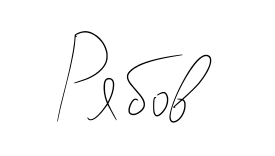
\includegraphics[width=2cm]{Prepared}
	П.Е. Рябов
\end{figure}


\begin{figure}[H]
	Утверждаю:\\
	Первый заместитель\\
	руководителя департамента\\
	Дата 01.06.2021
	\hfill
	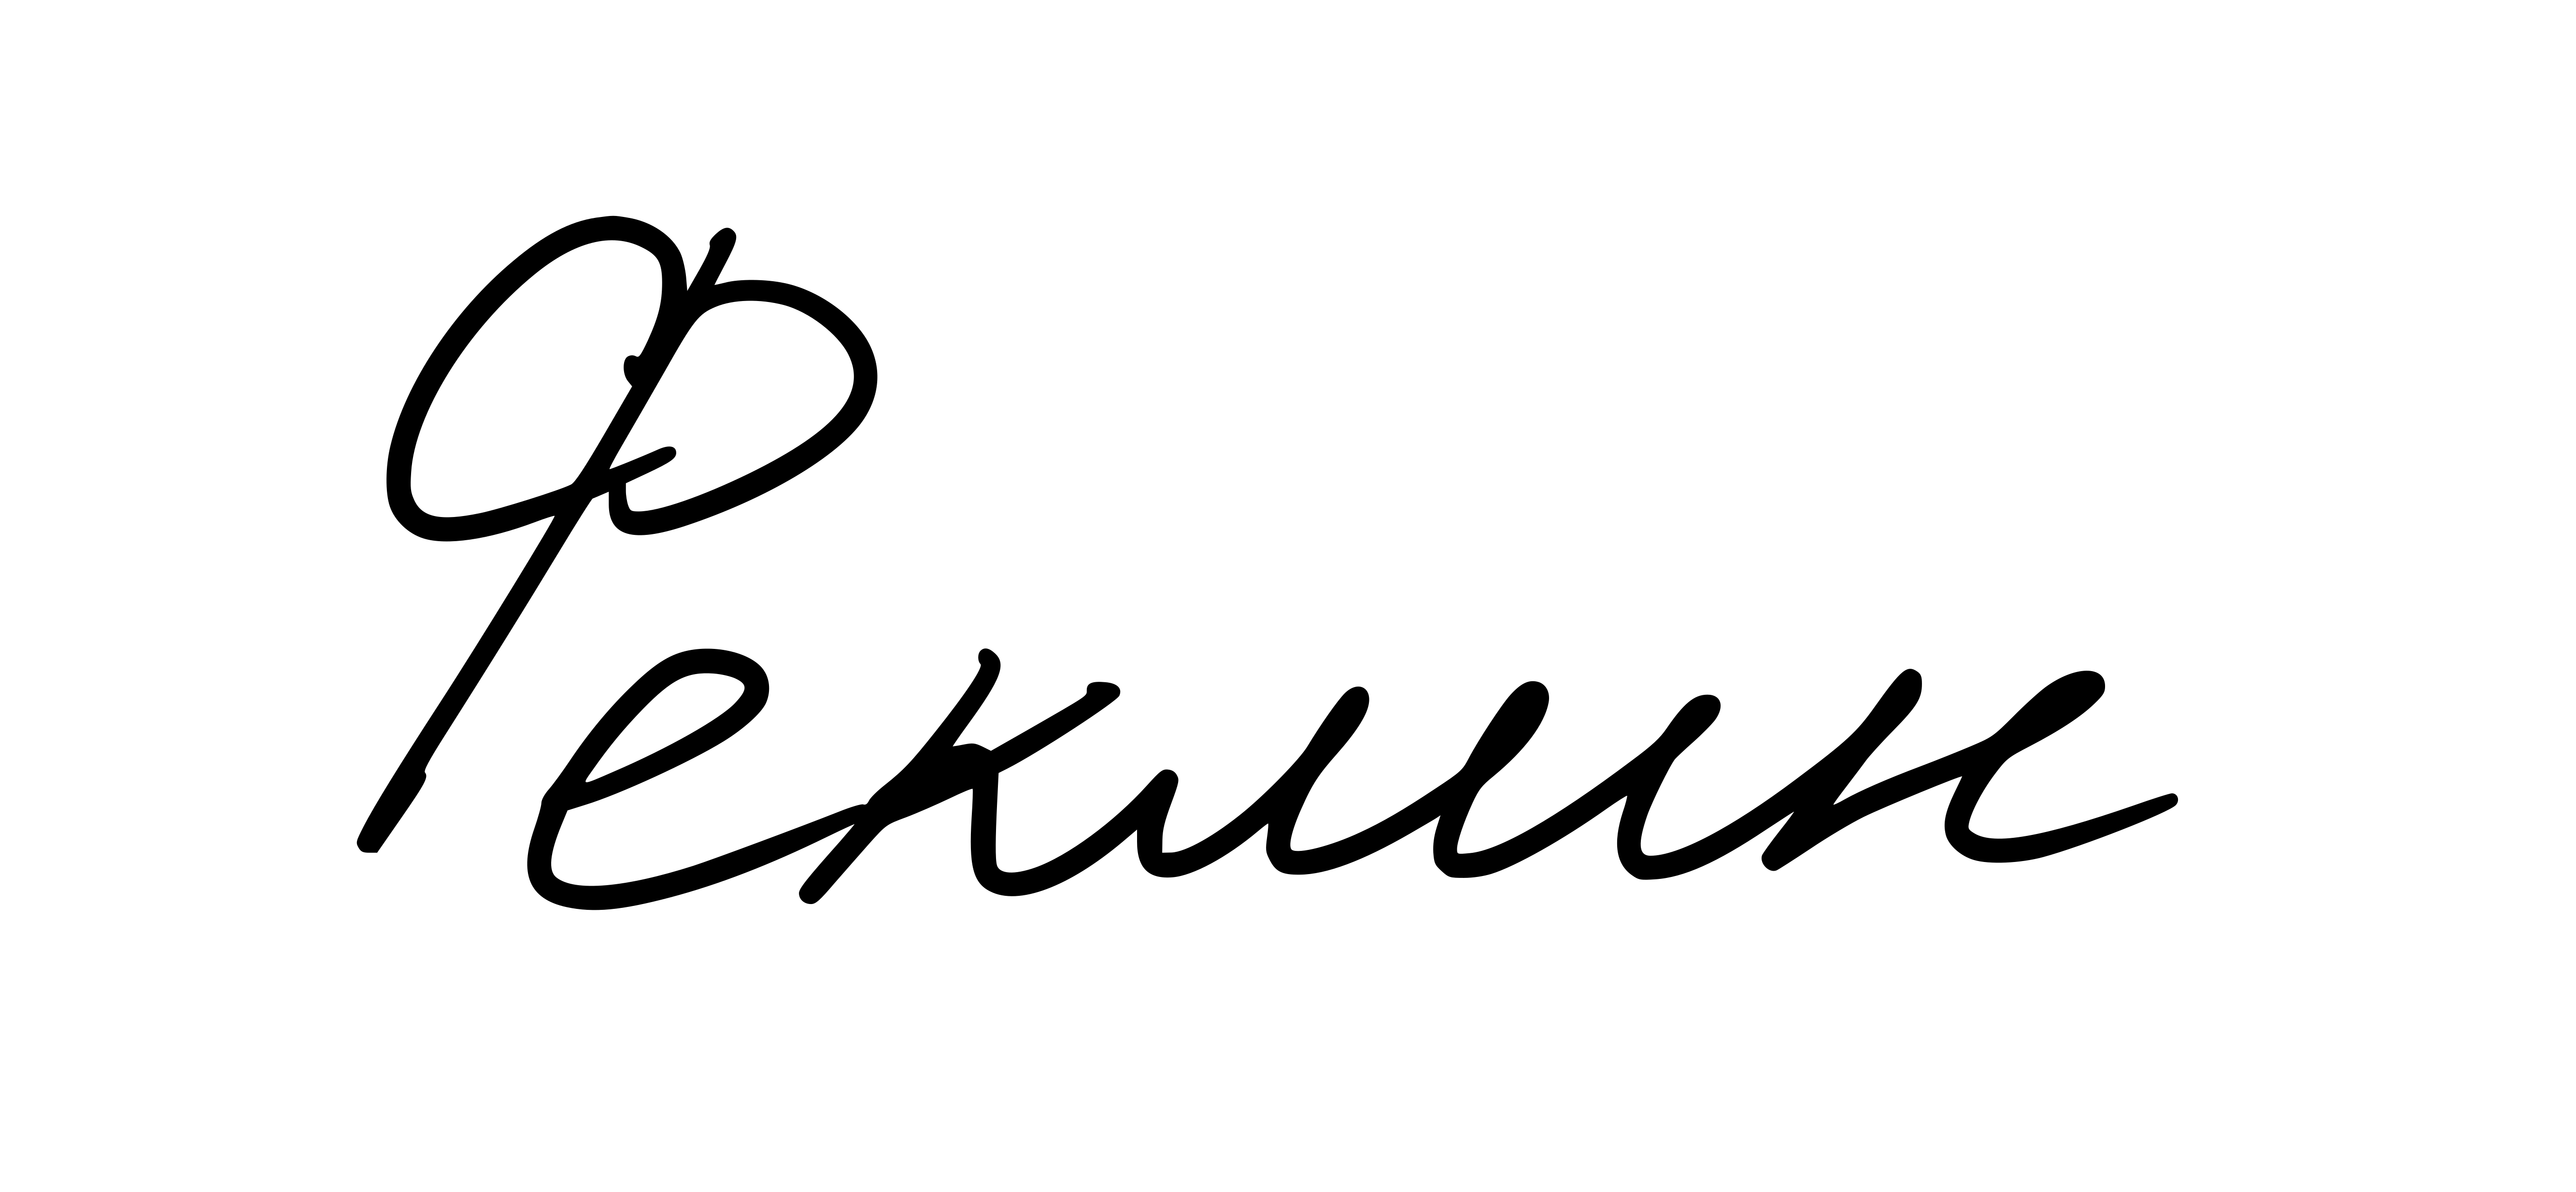
\includegraphics[width=2cm]{Approved}
	Феклин В.Г.
\end{figure}

\end{document}

